\begin{figure}[ht!]
    \centering
    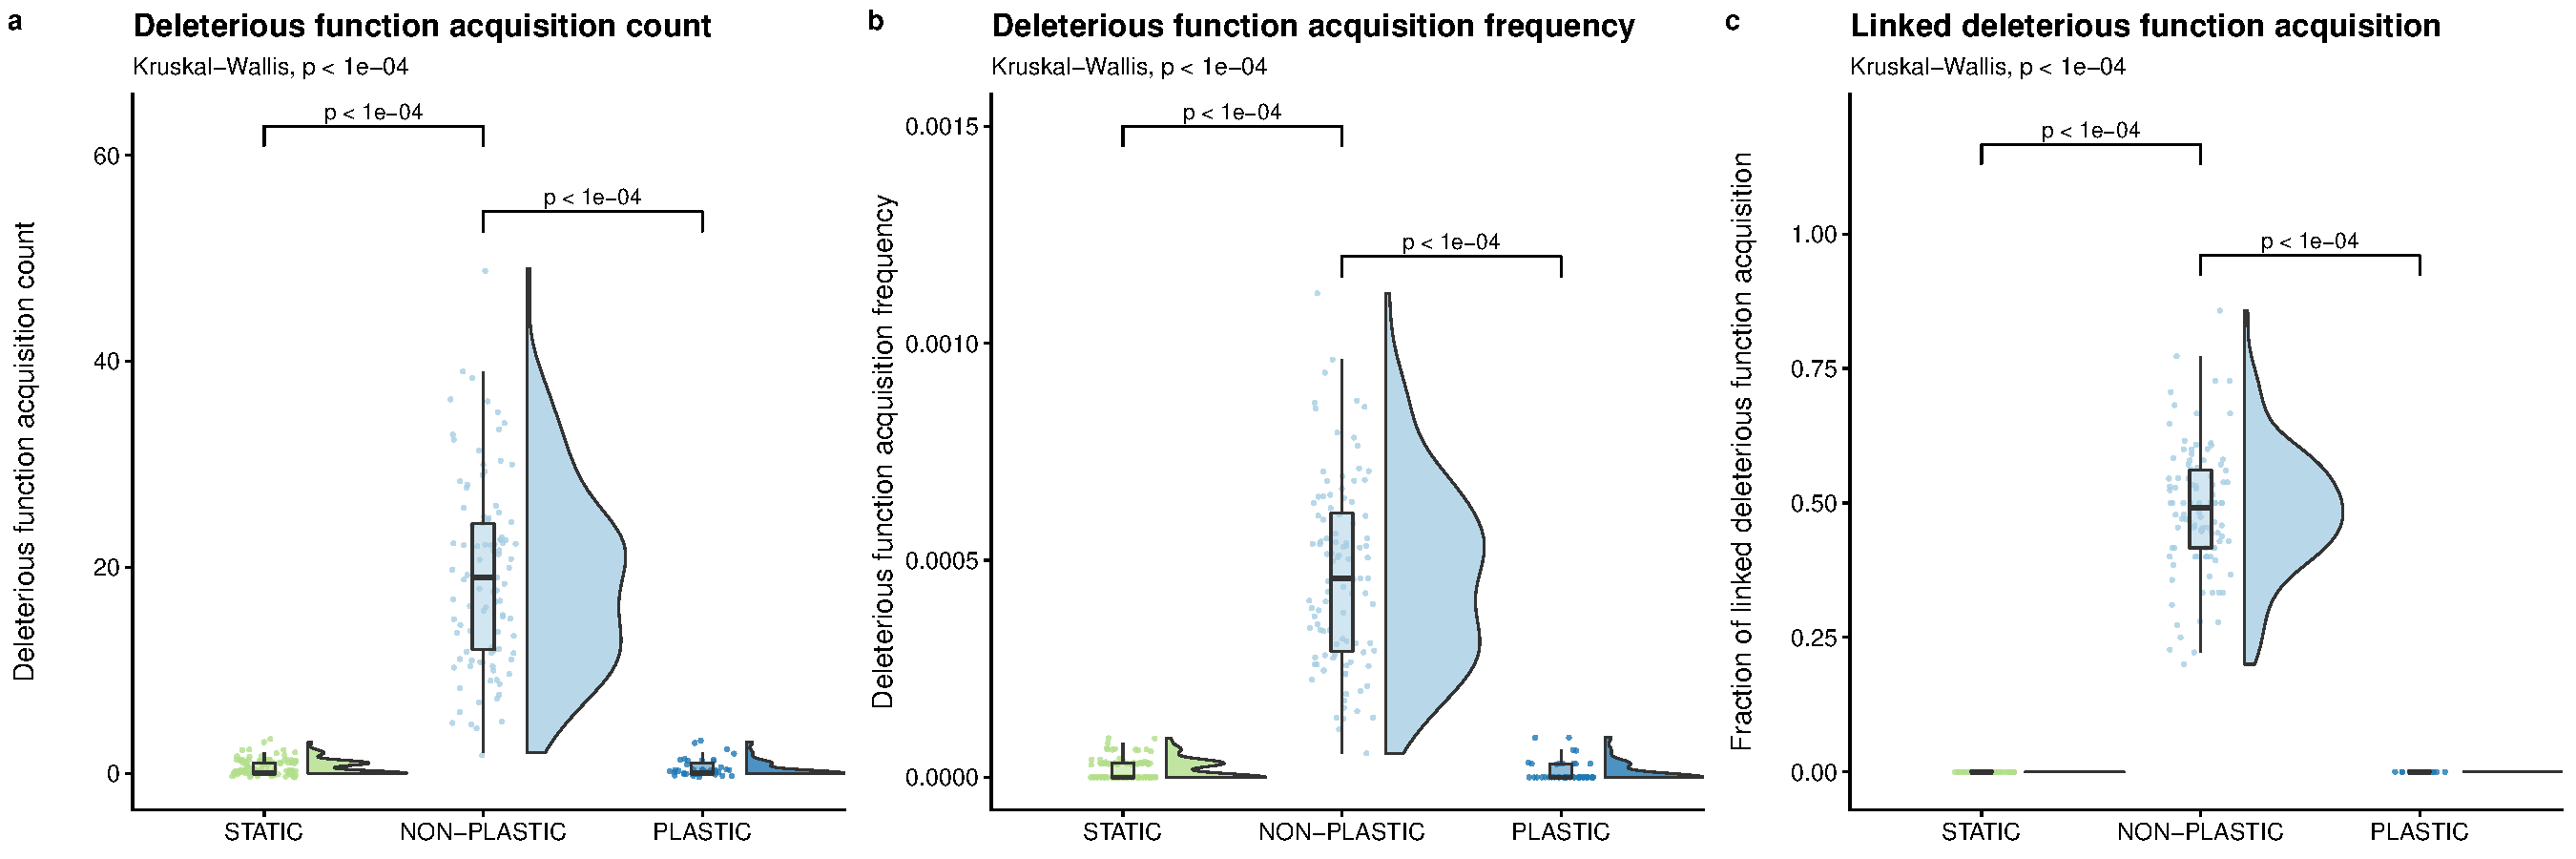
\includegraphics[width=1.0\textwidth]{media-poison-accumulation-panel.pdf}
    \caption{\small
    \textbf{Deleterious instruction accumulation.}
    Raincloud plots of
    (a) poisonous task acquisition,
    (b) poisonous task acquisition frequency,
    and (c) the proportion of mutations that increase poisonous task performance along a lineage that co-occur with a change in phenotypic profile.
    Each plot is annotated with statistically significant comparisons (Bonferroni-corrected pairwise Wilcoxon rank-sum tests).
    Note that adaptive phenotypic plasticity evolved in \deleteriousHitchhikingPlasticReps\ of \deleteriousHitchhikingReplicates\ replicates from the PLASTIC treatment during phase one of this experiment; we used this more limited group to seed the \deleteriousHitchhikingPlasticReps\ phase-two PLASTIC replicates.
    }
    \label{fig:deleterious-hitchhiking}
\end{figure}